\chapter{Introduction \label{chap:intro}}
    
    \section{Motivation}
    
    % General Context    
    Approximately 71\% of the Earth is covered by waters and important tasks happen on them such as environment monitoring, merchandise interchange, and navigation and exploration. 
    Some of this tasks can be dangerous, exhaustive or tedious for humans, so a trend is the development and usage of automated and autonomous systems for executing these tasks. Thus, driven by military, scientific and commercial interests, the development of \acp{USV} has become a current demand \cite{Liu2016Unmanned}.
    
    Current \acp{USV} applications include: environment monitoring \cite{Caccia2005Sampling}; ocean resources exploration as oil and gas exploration \cite{Pastore2010Improving}; port, harbor and coastal surveillance for military purposes \cite{Caccia2007unmanned, Pastore2010Improving, Svec2011aAutomated}; transportation \cite{Kiencke2005Impact}; and scientific research \cite{Yan2010Development}.
    
    % Definition of USV
    \acp{USV} recalls a category of marine robots that act without crew on the water surface presenting autonomous behavior or being remotely controlled. In the last decades several techniques have been applied for making \acp{USV} autonomous, main challenges are related to collision avoidance, precisely navigation on the seagoing, and accordance to international marine rules (\ac{COLREGS}).
    
    % Collision Avoidance
    The \acs{COLREGS} determines rules that must be followed by maritime pilots for preventing collisions in potential collision scenarios such as crossing, head-on and overtaking. Currently, direct collision between ships represents 60\% of the accidents in the sea, and 56\% of the collisions are caused by \acs{COLREGS} violation \cite{Liu2016Unmanned, Campbell2012Review_COLREGs}. Thus, \ac{USV} must be compliant with the \ac{COLREGS} rules but the fact that \ac{COLREGS} were written by humans to humans using subjective and ambiguous terms generated dependency on human interpretation, implying a considerable challenge for \acp{USV} systems.
    
    % Proposed work
    In this thesis, we present a \ac{COLREGS}-compliant \ac{USV} guidance system capable of avoiding collision with static and dynamic obstacles. The development will be done using \ac{ROS} \cite{Quigley2009ROS} while the system validation and evaluation will be done through software simulation using the USV\_SIM simulator \cite{Paravisi2018Toward}.% and on field tests using the Platypus Lutra airboat \cite{PlatypusLutraAirboat}. 
    
    \section{Research Question, Objectives and Assumptions}
    
    \subsection{Research Question}
    
    The main problem we want to study is the development of COLREGs-compliant guidance system for navigation of autonomous robots in the water surface, namely \acp{USV}. We want to understand how this can be done, what are the known solutions and methods, and how the robot architecture must be. With this in mind, the research question for this thesis is as follows:

    How to develop a COLREGs-compliant \ac{USV} guidance system to perform autonomous tasks in the water surface?
    
    \subsection{Objectives}
    
    Provoked by the research question we defined the following specific objectives:
    
    \begin{enumerate}
        \item Study of related works for identification of known solutions and methods for COLREGs-compliant autonomous marine robots;
        \item Design of a COLREGs-compliant guidance system for autonomous marine robot;
        \item Implement the designed system - previous objective - using \ac{ROS};
        \item Test and Evaluate the developed system using the USV\_SIM simulator.
    \end{enumerate}
    
    \section{Main Contributions}
    
    The main contributions of this thesis are:
    \begin{itemize}
        \item A review of related works about the subject;
        \item A USV\_SIM integrated ROS package for COLREGS-compliant guidance of \ac{USV}.
    \end{itemize}

    % \section{Limitations}
    \section{Thesis Outline}
    
    % Thesis Outline
    In Chapter \ref{chap:2_TheoreticalBackground}, we present important definitions and background information related to our research. In Chapter \ref{chap:3_LiteratureReview}, we present and discuss the literature related to \acp{USV} guidance systems. 
    In Chapter \ref{chap:4_COLREGS_Compliant_Guidance_System}, we present the developed systems, its architecture, features and implementation. In Chapter \ref{chap:5_Simulation_And_Results}, we present simulation scenarios and results. In Chapter \ref{chap:6_Conclusion}, we discuss the retrieved results.
    
    
    In this chapter, the main aspects of the proposed 1-year long research project is presented. We present the research questions and objectives defined to guide our research plan, and the defined activities to answer the research questions and accomplish the objectives. Moreover, we present preliminary work and current academic progress.
    
    \section{Problem Statement}
    \label{sec:problem_statement}

    Our focus is to study, design and develop a guidance system for \acfp{USV} capable of avoid collision with obstacles and other vessels being in accordance with the \ac{COLREGS}.

    \section{Research Questions and Objectives}
    \label{sec:Research_Questions_and_Objectives}

    
        Motivated by the interest in understanding and develop a \ac{USV} guidance system we defined the following research questions to guide our research:
        
        \begin{center}
        \begin{itemize}
        % VJ Ver próximo comentário. Não é uma pergunta que requer "?" deves escrever como se fosse. Ex.: How are USV guidance systems developed?
        % DJ: Done
        \item [\textbf{Q1.}] How are \ac{USV} guidance systems developed?
            \begin{itemize}
            \item [\textbf{Q1a.}] What is a \ac{USV} guidance system composed of?
            \item [\textbf{Q1b.}] What are the state-of-the-art methods used for \ac{USV} guidance implementation?
            \end{itemize}
        % VJ Não tenho certeza se isso é uma pergunta em Inglês. Creio que não pois falta a inversão do sujeito. Talvez fique melhor assim: How are COLREGS-complaint collision avoidance techniques implemented?
        % DJ: Done
        \item [\textbf{Q2.}] How are \ac{COLREGS}-complaint collision avoidance techniques implemented?
            \begin{itemize}
            \item [\textbf{Q2a.}] What are the current \ac{COLREGS}-compliant techniques in use to avoid collisions?
            % \item [\textbf{Q2b.}] How could an \ac{USV} guidance system address \ac{COLREGS} ambiguity and subjectivity?
            \end{itemize}
        \end{itemize}
        \end{center}
        
        In addition to answering the research questions presented above we have the following objectives in our research:
        \newline
        
        \begin{center}
        \begin{itemize}
            \item Primary Objective:
                \begin{itemize}
                    \item [\textbf{POBJ1}] Implementation or integration of path planners and collision avoidance strategies for development of a \ac{COLREGS}-compliant guidance system for \ac{USV}.
                \end{itemize}
            \item Secondary Objectives:
                \begin{itemize}
                    \item [\textbf{SOBJ1}] Implementation of the system using \acf{ROS} \cite{Quigley2009ROS};
                    \item [\textbf{SOBJ2}] Simulation of the system using USVSIM \cite{Paravisi2018Toward};
                    \item [\textbf{SOBJ3}] Test on field using Platypus Lutra airboat \cite{PlatypusLutraAirboat}.
                \end{itemize}
        \end{itemize}
        \end{center}

    \section{Activities and Schedule}
    \label{subsec:activities_and_schedule}
        % VJ "and comply with the graduate course? This is new... nunca vi ninguém esrevendo isso numa proposta de pesquisa. Talvez seja melhor tirar."
        %AMA 31/1 um tanto estranho mesmo. Keet it Simple ! The activities for 2019 are presented as follows:   ... ou algo similar da sua escolha
        % DJ: Done.
        The activities and schedule (\ref{tab:schedule}) for 2019 are presented as follows::
        
        \begin{enumerate}
            % VJ Eu tiraria o que vêm depois dos dois pontos desta linha.
            % DJ: Done.
            \item \textbf{Researh Plan - Writing and Presentation};
            
            % VJ Loooong sentences. Quebra elas em pedaços menores
            % DJ: Done.
            \item \textbf{\ac{USV} Guidance System State-Of-The-Art Mapping} 
            
            This activity consists of the research of studies related to the development of \ac{USV} guidance systems for USVs and the generation of a document that presents a mapping of techniques used for implementation of global and local guidance systems and the implementation of COLREGS-compliant systems. Moreover, we want to identify metrics used for evaluation of the developed systems.
            
            The search for related work will be performed through snowballing~\cite{Wohlin2014Guidelines} from the most relevant surveys related to \ac{USV} guidance, collision avoidance, and \ac{COLREGS} compliance. All captured information will be arranged in text and a table similar to Table \ref{tab:RelatedWork_Summary}. This activity addresses research questions \textbf{Q1a}, \textbf{Q1b}, and \textbf{Q2a};
            % VJ Troquei o potentially allow (gramaticamente incorreto pois deveria ser singular: allows) por addresses. E tirei o "the result of". Se achares ruim, modifique.
            % DJ: Accepted.
            
            % VJ Reescrever. Fiquei em dúvida se vc estava se referindo a sua própria técnica ou uma técnica do estado da arte. Lembre-se, e isso vai te ajudar  reescrever, _você_ vai desenvolver um "método de guidance". Quando vc usa "selection of methods" você não especifica nada e o leitor tem que inferir de quê. Isso em geral é ruim, pois dependendo do que o leitor está pensando -- o seja, ele poe se confundir. 
            % VJ Pra mim são duas atividades separadas: implementar a técnica que representa o estado da arte; e propor uma nova técnica estudando as limitações e pontos fortes de cada trabalho.
            % VJ Com respeito à novelty, me lembrei de uma coisa. Eles vão te perguntar porque não implementar uma técnica existente. Pelos estudos que você realizou até agora, existem poucas comparações de técnicas em testes reais e além disso, poucas implementações completas disponíveis. Em parte isso se deve a pouca disponibilidade de sistemas completos para teste. A PUCRS dispõe do hardware. Por fim, como há pouca ou nenhuma comparação entre técnicas, AFAIK, e isso pode indicar que ainda há problemas nas técnicas implemetadas que ainda não foram identificados. Liste as novidades do que vc vai fazer. Uma écnica melhor, umaa comparação de técnicas usando USVs em testes reais, etc.. Essa parte tem pouco a ver com esta sessão, mas eu escrevi aqui pois foi aqui que me caiu a ficha. Acho que cabe falar sobre isso no 1o capítulo.
            
            % DJ: Conversando com o prof. Amory concluimos que concordamos contigo mas isso não será "vendido" nesta versão da proposta.
            
            \item \textbf{Design and Implementation of a \ac{COLREGS}-compliant \ac{USV} Guidance System based on the State-Of-The-Art}
            
            This activity consists of the selection, design, and implementation of guidance methods to compose our \ac{COLREGS}-compliant \ac{USV} guidance system. Both guidance methods and guidance system architecture will be defined based on the information captured in activity 2. The guidance system will be developed using \ac{ROS}. Thus, this activity will be developed using the information captured on acitivty 2. As deliverable, activity 3 generates the implementation code of the \ac{USV} \ac{COLREGS}-compliant guidance system. Activity 3 addresses objectives \textbf{POBJ1} and \textbf{SOBJ1}.
            %AMA 31/1 nao entendi essa parte. o que eh o entregavel dessa atividade ? eu havia entendido q era codigo / programa, mas aqui vc diz q eh texto e tabelas ?!?!?
            %AMA 31/1 enumera os objetivos tipo OBJ1. acho q facilita a cross ref. 
            % DJ: Done.
            
            \item \textbf{Simulation and Evaluation of the Implemented System} 
            
            This activity consists of the simulation of the \ac{COLREGS}-compliant \ac{USV} guidance system developed in activity 3 using the USVSIM simulator presented in Section \ref{sec:usvsim}. This activity embraces the definition, development, and execution of test scenarios. The scenarios will be developed to test and validate the correct behavior on performing global and Local collision avoidance with static and dynamic obstacle following \ac{COLREGS} rules 13 - Overtaking, 14 - Head-On, 15 - Crossing, and 16/17 - Action by Stand-on/Give-way vessel. The evaluation will be done using identified metrics on the activity 2.
            %AMA 31/1 acti 2 nao menciona metrics. arruma la pois eh importante identifica-las. 
            % DJ: Done
            
            % VJ Penso que dizer isso é prematuro pois depende do sensor que vc vai usar, 
            
            %AMA 31/1 nesse ponto (baseado em sim) penso q ele pode abstrair os sensores usados p perceber os obstaculos. eu discuti algumas estrategias c o darlan. pede p ele discutir contigo isso. Claro, qnd for p o barco real ele vai ter q ter essa camada adiciona do software q eh dependente dos sensores
            
            % que aliás me parece que ainda está em aberto. Por exemplo, vc poderia simular um lidar facilmente para testes em simulação. Cuidado. As simulações vão sim envolver simulação de sensores em algum momento antes de meter teu método na água. Precisamos conversar sobre isso.
            % VJ Vc não vai usar apena tópicos, pode vir a ter que implementar um ROSService
            In simulation scenarios, as a first step, we will simulate the obstacle detection directly getting the information about obstacles provided by the USVSIM simulator (through \ac{ROS} topics/services messages). As a second step, we will add real sensors to the simulation to ease future integration with real-boat. Thus, activity 4 addresses objective SOBJ2; 
            
            \item \textbf{Progress Seminar - Writing and Presentation};
            
            % VJ prematuro falar de sensores. Não faça este tipo de commitment. Seja mais genérico ao falar de sensores, podes usar o termo sensores exteroceptivos disponíveis, use-os apenas como exemplos. Acho que vale a pena mudar aqui e na parte de simulação.
            % VJ Empirically tuned PID? Tira isso. Fica feio escrever isso já na proposta
            % VJ para escolher entre "an" e "a" em acrônimos vc deve levar em conta como o mesmo é pronunciado e não a letra que vem primeiro ser consoante ou vogal. Por isso, a forma correta é "anargibidi camera" :D
            % DJ: Done.
            \item \textbf{Integration with Real-Boat}
            
            This activity is the first step for tests on fields, it embraces necessary integration for execution of the developed system on the real-boat hardware. For tests on the real world, the perception system will be composed of available exteroceptive sensors (eg. \ac{RGBD} camera, and \ac{LIDAR}), the navigation system will be composed by compass, \ac{GPS}, and barometer, and the control system will be implemented through a \ac{PID}. So, as deliverable we will gerenate the adapted \ac{ROS} code to use real sensors and actuators. Thus, activity 6 addresses objective SOBJ3;
            % VJ Sugestão: Esta etapa é o passo tal para testar o sistema em ambientes reais -- the next activity
            %AMA 31/1 aqui acho q eh bom dar mais enfase nos desafios q serao encontrados pois vai ser um passo bem grande sair do simulador p o barco, ainda mais q no simulador a percepcao vai ser 'abstraida'. deiaxar claro q o foco vai ser em desenvolver (nao necessariamente, se for possivel reusar algo) ou integrar o foco de percepcao.
            % DJ: Partially done but probably not detailed enough yet.
            
            % VJ Evaluate through the evaluation...
            % VJ Through the evaluation of the reactive actions chosen. Acho que isso é desnecessário ou incompleto. Ou você tira/modifica ou escreve mais. Colisão é uma forma de avaliação, por exemplo. Distância e caminho escolhido também. Suavidade, etc.
            % VJ Sugestão use o número dos bullets ao invés de escrever "the first seconday objective". Vai ficar muito mais simples de escrever tudo.
            % DJ: Done
            \item \textbf{Real-Boat Test and Evaluation}
            
            This activity consists of the reconstruction of the simulated scenarios for tests in the real world. For this purpose, we will use two \ac{USV}, one with the developed guidance system and another remotely controlled, this way we are going to simulate possible collision scenarios between the vessels (head-on, overtaking, crossing) and evaluate the behavior of our guidance system rating the reactive actions chosen. Some criterion are chosen way, \ac{COLREGS}-compliance, minimun distance related to the obstacle, and path smoothness. Thus, activity 7 addresses the objective SOBJ3;
            
            %AMA 31/1 vc consegue imaginar como vai ser realizada essa avaliacao ? se sim, escreva um pouco. q metrica vc vai usar p dizer q metodo X eh melhor q metodo Y ? vc vai precisar de equiapamentos especializados ? 
            
            % \item \textbf{Investigation of New Strategies for \ac{COLREGS} Compliance Implementation (optional)};
            % \item \textbf{Design and Implementation a New Strategy for \ac{COLREGS} Compliance Implementation (optional)};
            % \item \textbf{Simulation and Evaluation a New Strategy for \ac{COLREGS} Compliance (optional)};
            % \item \textbf{Adaptation of a New Strategy for \ac{COLREGS} Compliance Implementation (optional)};
            % \item \textbf{Real-Boat Test and Evaluation of a New Strategy for \ac{COLREGS} Compliance (optional)};
            
            \item \textbf{Dissertation - Writing and Presentation}.
        \end{enumerate}

        % \begin{landscape}
        \begin{table}[H]
        \caption{Proposed Schedule}
        \label{tab:schedule}
        \centering
        \begin{tabular}{|c|cccccccccccc|}
        \hline
        Activity & \textbf{Jan}                                  & \textbf{Feb}                                  & \textbf{Mar}                                  & \textbf{Apr}                                  & \textbf{May}                                  & \textbf{Jun}                                  & \textbf{Jul}                                  & \textbf{Aug}                                  & \textbf{Sep}                                  & \textbf{Oct}                                  & \textbf{Nov}                                  & \textbf{Dec} \\ \hline
        1        & \multicolumn{1}{c|}{\cellcolor[HTML]{000000}} & \multicolumn{1}{c|}{}                         & \multicolumn{1}{c|}{}                         & \multicolumn{1}{c|}{}                         & \multicolumn{1}{c|}{}                         & \multicolumn{1}{c|}{}                         & \multicolumn{1}{c|}{}                         & \multicolumn{1}{c|}{}                         & \multicolumn{1}{c|}{}                         & \multicolumn{1}{c|}{}                         & \multicolumn{1}{c|}{}                         &              \\ \cline{2-13} 
        2        & \multicolumn{1}{c|}{}                         & \multicolumn{1}{c|}{\cellcolor[HTML]{000000}} & \multicolumn{1}{c|}{\cellcolor[HTML]{000000}} & \multicolumn{1}{c|}{}                         & \multicolumn{1}{c|}{}                         & \multicolumn{1}{c|}{}                         & \multicolumn{1}{c|}{}                         & \multicolumn{1}{c|}{}                         & \multicolumn{1}{c|}{}                         & \multicolumn{1}{c|}{}                         & \multicolumn{1}{c|}{}                         &              \\ \cline{2-13} 
        3        & \multicolumn{1}{c|}{}                         & \multicolumn{1}{c|}{}                         & \multicolumn{1}{c|}{\cellcolor[HTML]{000000}} & \multicolumn{1}{c|}{\cellcolor[HTML]{000000}} & \multicolumn{1}{c|}{\cellcolor[HTML]{000000}} & \multicolumn{1}{c|}{}                         & \multicolumn{1}{c|}{}                         & \multicolumn{1}{c|}{}                         & \multicolumn{1}{c|}{}                         & \multicolumn{1}{c|}{}                         & \multicolumn{1}{c|}{}                         &              \\ \cline{2-13} 
        4        & \multicolumn{1}{c|}{}                         & \multicolumn{1}{c|}{}                         & \multicolumn{1}{c|}{}                         & \multicolumn{1}{c|}{}                         & \multicolumn{1}{c|}{}                         & \multicolumn{1}{c|}{\cellcolor[HTML]{000000}} & \multicolumn{1}{c|}{\cellcolor[HTML]{000000}} & \multicolumn{1}{c|}{}                         & \multicolumn{1}{c|}{}                         & \multicolumn{1}{c|}{}                         & \multicolumn{1}{c|}{}                         &              \\ \cline{2-13} 
        5        & \multicolumn{1}{c|}{}                         & \multicolumn{1}{c|}{}                         & \multicolumn{1}{c|}{}                         & \multicolumn{1}{c|}{}                         & \multicolumn{1}{c|}{}                         & \multicolumn{1}{c|}{}                         & \multicolumn{1}{c|}{\cellcolor[HTML]{000000}} & \multicolumn{1}{c|}{}                         & \multicolumn{1}{c|}{}                         & \multicolumn{1}{c|}{}                         & \multicolumn{1}{c|}{}                         &              \\ \cline{2-13} 
        6        & \multicolumn{1}{c|}{}                         & \multicolumn{1}{c|}{}                         & \multicolumn{1}{c|}{}                         & \multicolumn{1}{c|}{}                         & \multicolumn{1}{c|}{}                         & \multicolumn{1}{c|}{}                         & \multicolumn{1}{c|}{}                         & \multicolumn{1}{c|}{\cellcolor[HTML]{000000}} & \multicolumn{1}{c|}{}                         & \multicolumn{1}{c|}{}                         & \multicolumn{1}{c|}{}                         &              \\ \cline{2-13} 
        7        & \multicolumn{1}{c|}{}                         & \multicolumn{1}{c|}{}                         & \multicolumn{1}{c|}{}                         & \multicolumn{1}{c|}{}                         & \multicolumn{1}{c|}{}                         & \multicolumn{1}{c|}{}                         & \multicolumn{1}{c|}{}                         & \multicolumn{1}{c|}{}                         & \multicolumn{1}{c|}{\cellcolor[HTML]{000000}} & \multicolumn{1}{c|}{}                         & \multicolumn{1}{c|}{}                         &              \\ \cline{2-13} 
        8        & \multicolumn{1}{c|}{}                         & \multicolumn{1}{c|}{}                         & \multicolumn{1}{c|}{}                         & \multicolumn{1}{c|}{}                         & \multicolumn{1}{c|}{}                         & \multicolumn{1}{c|}{}                         & \multicolumn{1}{c|}{}                         & \multicolumn{1}{c|}{}                         & \multicolumn{1}{c|}{}                         & \multicolumn{1}{c|}{\cellcolor[HTML]{000000}} & \multicolumn{1}{c|}{\cellcolor[HTML]{000000}} &              \\ \hline
        \end{tabular}
        \end{table}
        % \end{landscape}
       
       %AMA 31/1 nao carece essas cores. parecem sem proposito.  pode ser tudo preto mesmo
       % DJ: Done.
       
        
    % \section{Proposed Modeling for a First Trial}
    % \label{sec:proposed_modeling}
    
    %     Based on the study done until the writing of this research plan we defined a first trial model of a \ac{USV} \ac{COLREGS}-compliant guidance system. Following thme architecture presented by most of the read studies about \ac{USV}, we propose the usage of global and local guidance modules as main components of the \ac{USV} guidance system. We propose the usage of \acf{DPSS} for global guidance and \acf{R-RA*} for \ac{COLREGS}-compliant local guidance\footnote{Both methods are described in Chapter \ref{chap:3_StateOfTheArt}.}. We want our system to be in accordance with \ac{COLREGS} 13 - Overtaking, 14 - Head-On, and 15 - Crossing.
        
    %     With \ac{DPSS} our system will be capable of generating global path planning considering both static and dynamic obstacle. Trying to keep it simple, with \ac{R-RA*} our system will reactively generate collision avoidance trajectories through execution of a modification of the A*. As presented by Campbell \etal~\cite{Campbell2013Automatic}, the implementation of the \ac{COLREGS}-complaint behavior is done through state space constraining related to each one of the desired rules. We visualize the usage of a 2D map for representation of the environment through occupancy grid and information captured by a near-field perception system.
        
    %     For simulation, as a first trial, we want to simulate the obstacle detection directly getting the information about obstacles provided by the USVSIM simulator - through \ac{ROS} topics messages -, thus we will not simulate the hardware (\ac{LIDAR}, cameras, and others) of a perception system. For tests on the real world, our perception system will be composed of a \ac{RGBD} camera and a \ac{LIDAR}. Our navigation system will be composed of compass, \ac{GPS}, and barometer. Our control system will be implemented through an empiric tuned \ac{PID}.
    
    \section{Preliminary Work}
    \label{sec:Preliminary_Work}

    % VJ use mais artigos definidos e indefinidos
    % VJ an eidchTiEn
    As a deliverable for Intelligent Mobile Robotics and Automated Planning graduate courses, we addressed the problem of \ac{COLREGS}-compliant collision avoidance, and developed a \ac{POC} system composed of a \ac{USV} 3D simulator and an \ac{HTN} planner. The architecture of this \ac{POC} system is presented in Figure \ref{fig:USVSIM_JSHOP}. For the \ac{USV} 3D simulation we have used USVSIM \cite{Paravisi2018Toward}, while for the chosen \ac{HTN} planner was \ac{JSHOP}2~\cite{Nau2003SHOP2_System}.  \ac{JSHOP}2~\cite{Nau2003SHOP2_System} is the Java implementation of SHOP2 (Simple Hierarchical Ordered Planner). SHOP2 is a domain-independent automated-planning system. It is based on ordered task decomposition, which is a type of \acl{HTN} planning. So, \ac{JSHOP}2 is a modified version of \ac{HTN} planning that involves planning for tasks in the same order that they will be executed.
    
    In our system, from one side the USV\_GUIDER \cite{Darlan2018USV_GUIDER} is responsible for interpreting the plan generated by the \ac{JSHOP}2 and translate the defined actions into \ac{ROS} commands. The \ac{ROS} commands are linked to one boat. From the other side, the USV\_GUIDER is responsible for translate conditions of the simulated environment to a description compliant to the \ac{JSHOP}2 acceptable syntax. The conditions are directly captured through \ac{ROS} topics. 
    
    % VJ De novo o PID com parâmetros empíricos
    % DJ: Done.
    So, in our architecture, the \ac{HTN} planner is responsible for determination of which \ac{COLREGS} rule must be applied in a detected dangerous situation through evaluation of information captured by the perception system. The global guidance module of the guidance system is responsible for command the simulated \ac{USV} straight ahead continuously. The local guidance system is responsible for avoiding detected hazard situation guiding the \ac{USV} toward its starboard side. The control system is composed of a \ac{PID} to be capable of following guidance commands. The perception system is capable of detecting any obstacle in the near-field.
    
    \begin{figure}[H]
        \centering
        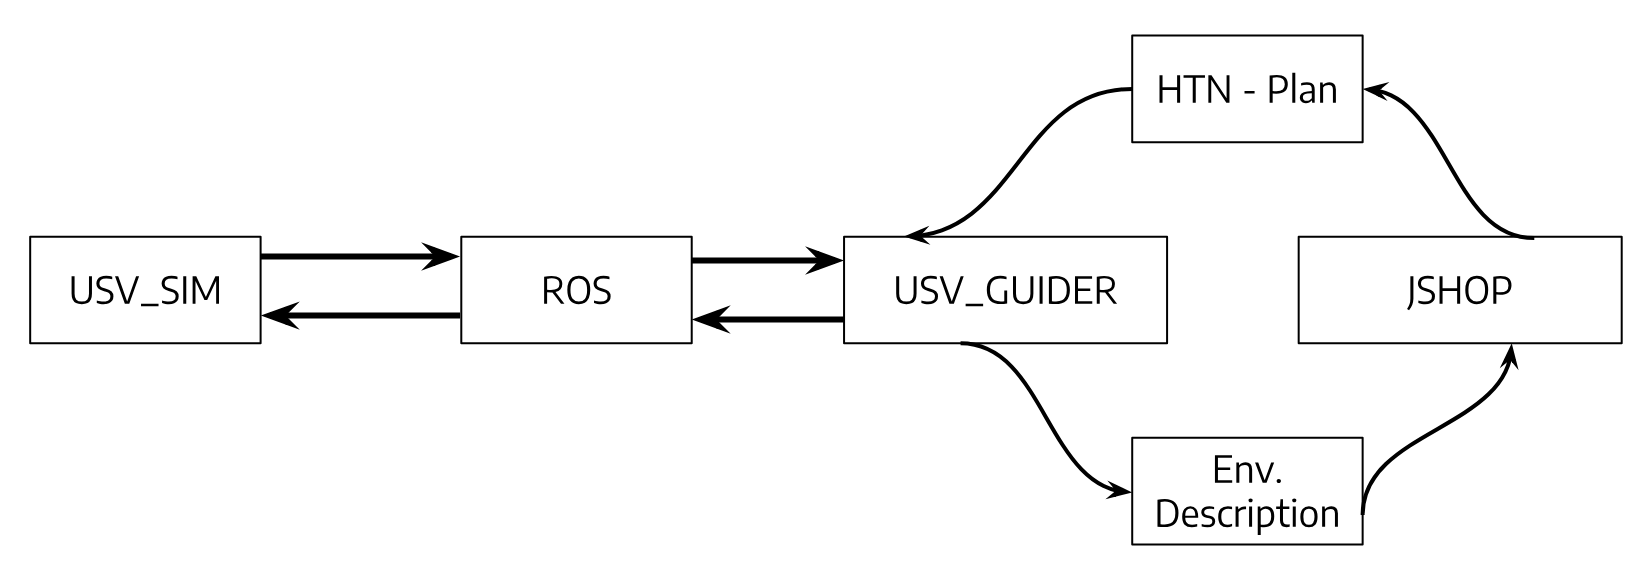
\includegraphics[scale=0.3]{figs/POC_USVSIM_JSHOP2.png}
        \caption{POC System}
        \label{fig:USVSIM_JSHOP}
    \end{figure}
    
    % VJ: Mexi aqui. Mas ainda me parece que vc está misturando info do JShop com o teu método. 
    The USV\_GUIDER was implemented in Python. \ac{JSHOP}2 is originally designed for user interaction through \ac{GUI}. For this integration, we have modified  \ac{JSHOP}2 so it could be executed from command prompt. This way, % the USV_GUIDER? se for substitui % DJ: Done.
    the USV\_GUIDER is capable of performing system calls to run \ac{JSHOP}2 when needed. Every execution of \ac{JSHOP}2 reinterprets the generated environment description and generates a new plan. This plan defines the guide command. Possible guide commands are: keep going straight ahead, turn left, turn right, accelerates 10\% related to current velocity, decelerates 10\% related to current velocity.  
    % VJ This plan...
    % DJ: Done.
    
    For validation of the integrated system was performed the simulation of a situation where one air-boat moves toward another anchored air-boat in a head-on situation. A boat following the \ac{COLREGS} must avoid the possible collision changing direction to its starboard side. Figure \ref{fig:COLREGs_HeadOn} illustrates the head-on situation. Figure \ref{fig:Experiments_HeadOn_InitialState} illustrates the initial state of the experiment. In this experiment, the controlled boat is expected to start sailing ahead, but change its direction once the risk of head-on collision is detected, as shown in Figure \ref{fig:Experiment_HeadOn_Sequence}. After evading the dangerous situation, the controlled boat returns to its straight-ahead sailing mode.
    % VJ modifiquei acima, mas o finalzinho poderia melhorar
    
    \begin{figure}[H] 
        \centering
        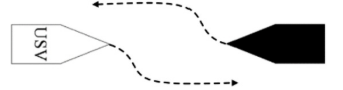
\includegraphics[scale=0.6]{figs/COLREGS_HeadOn.png}
        \caption{Experiment - Head-on}
        \label{fig:COLREGs_HeadOn}
    \end{figure}
    
    \begin{figure}[H] 
        \centering
        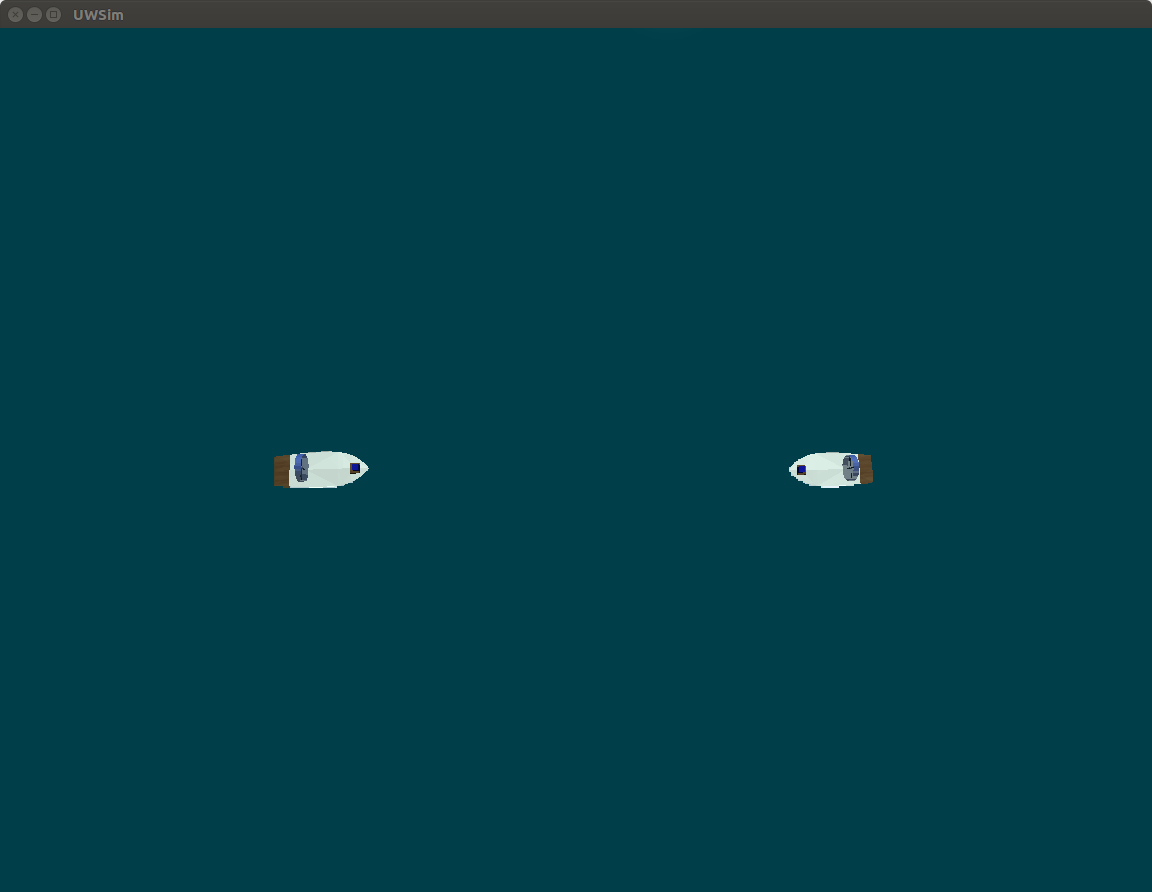
\includegraphics[scale=0.2]{figs/Experiment_HeadOn_1.png}
        \caption{Experiment - Head-on}
        \label{fig:Experiments_HeadOn_InitialState}
    \end{figure}
    
    \begin{figure}[H]
        \centering
        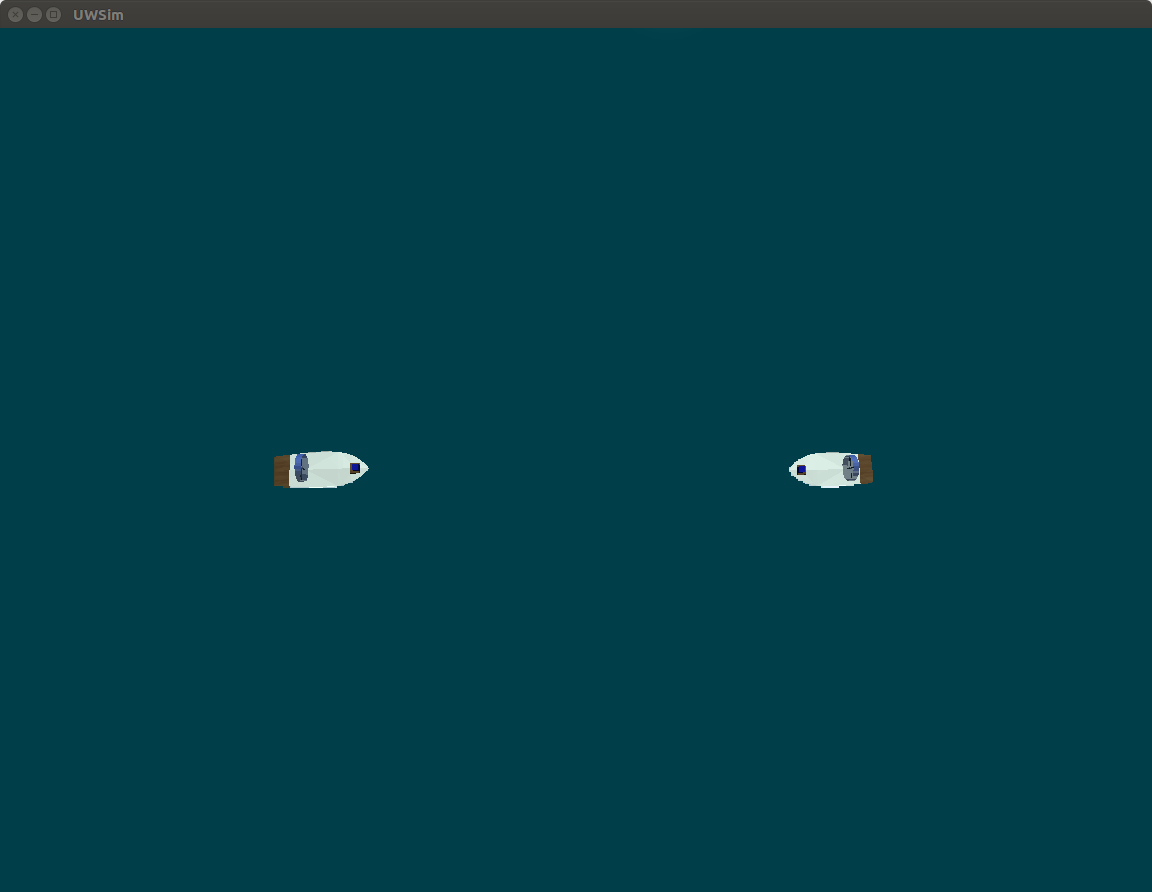
\includegraphics[scale=0.2]{figs/Experiment_HeadOn_1.png}
        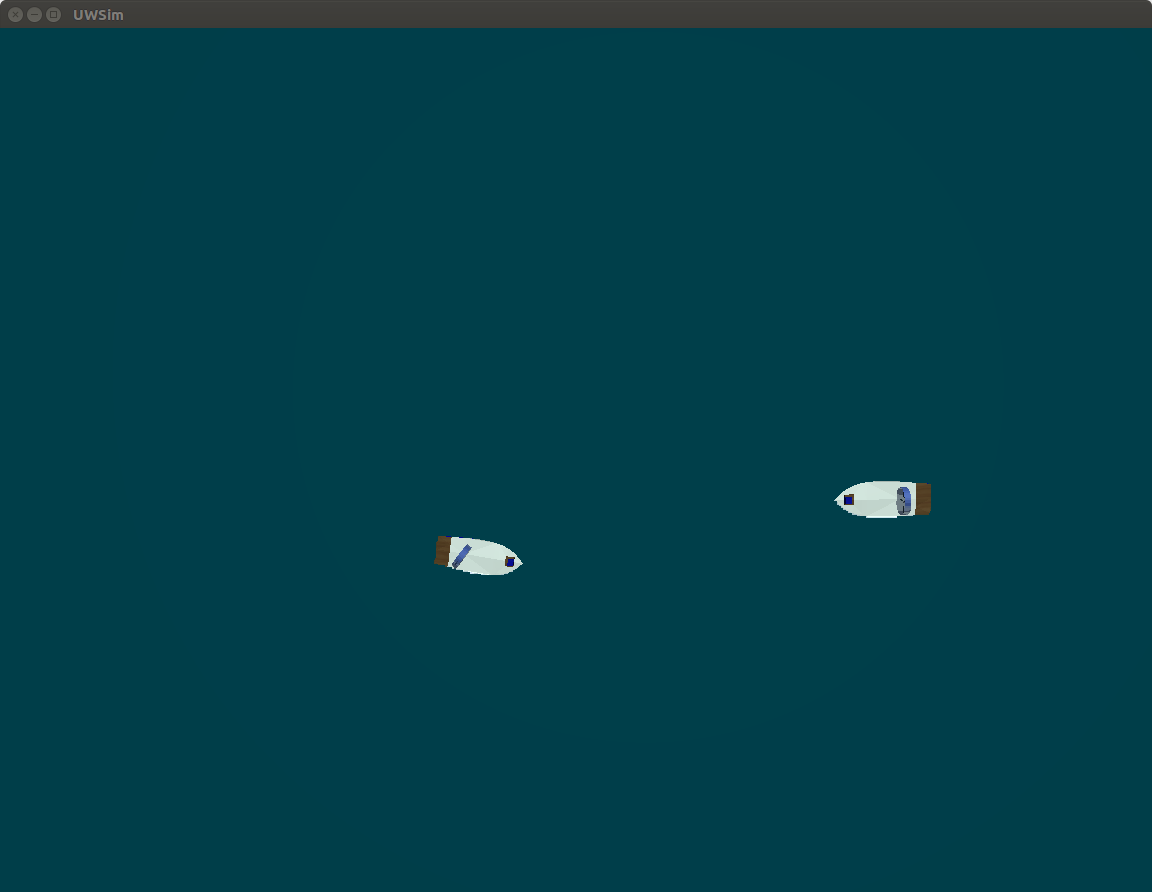
\includegraphics[scale=0.2]{figs/Experiment_HeadOn_3.png}\\
        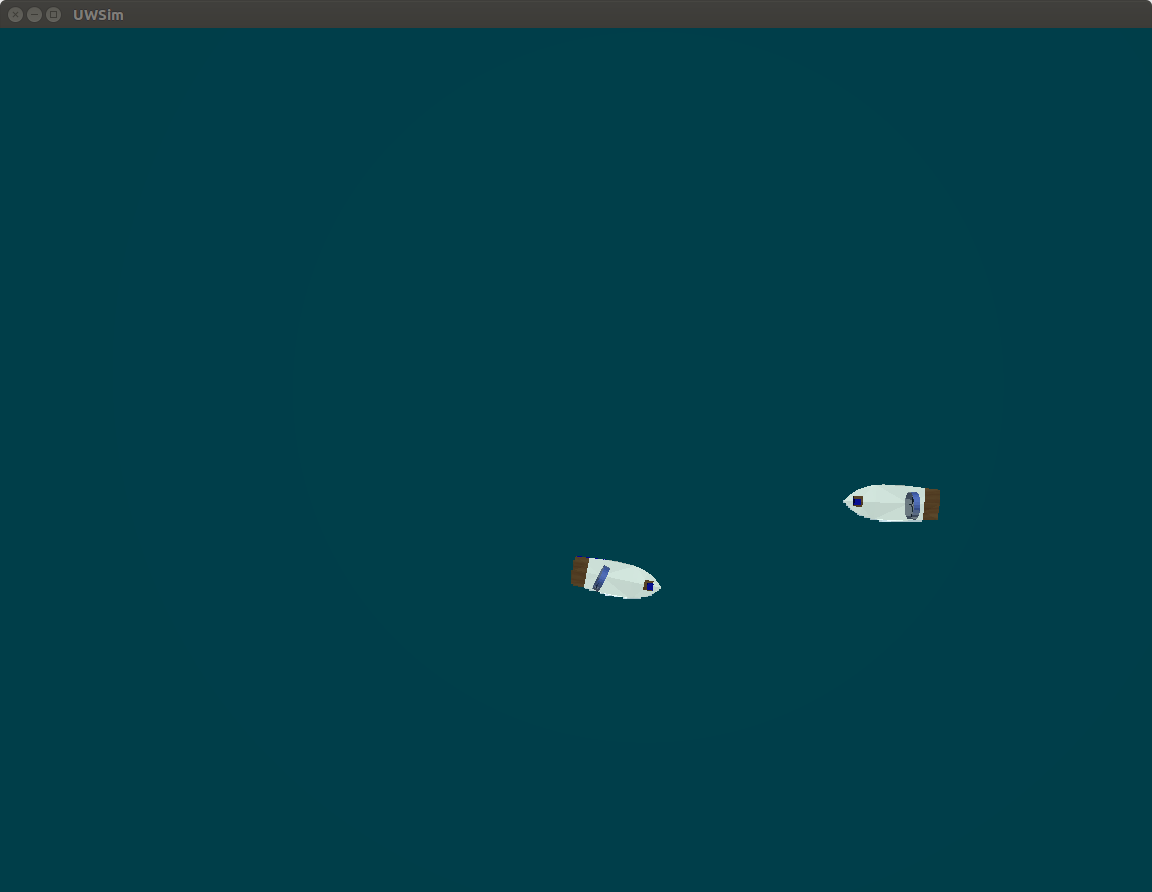
\includegraphics[scale=0.2]{figs/Experiment_HeadOn_4.png}
        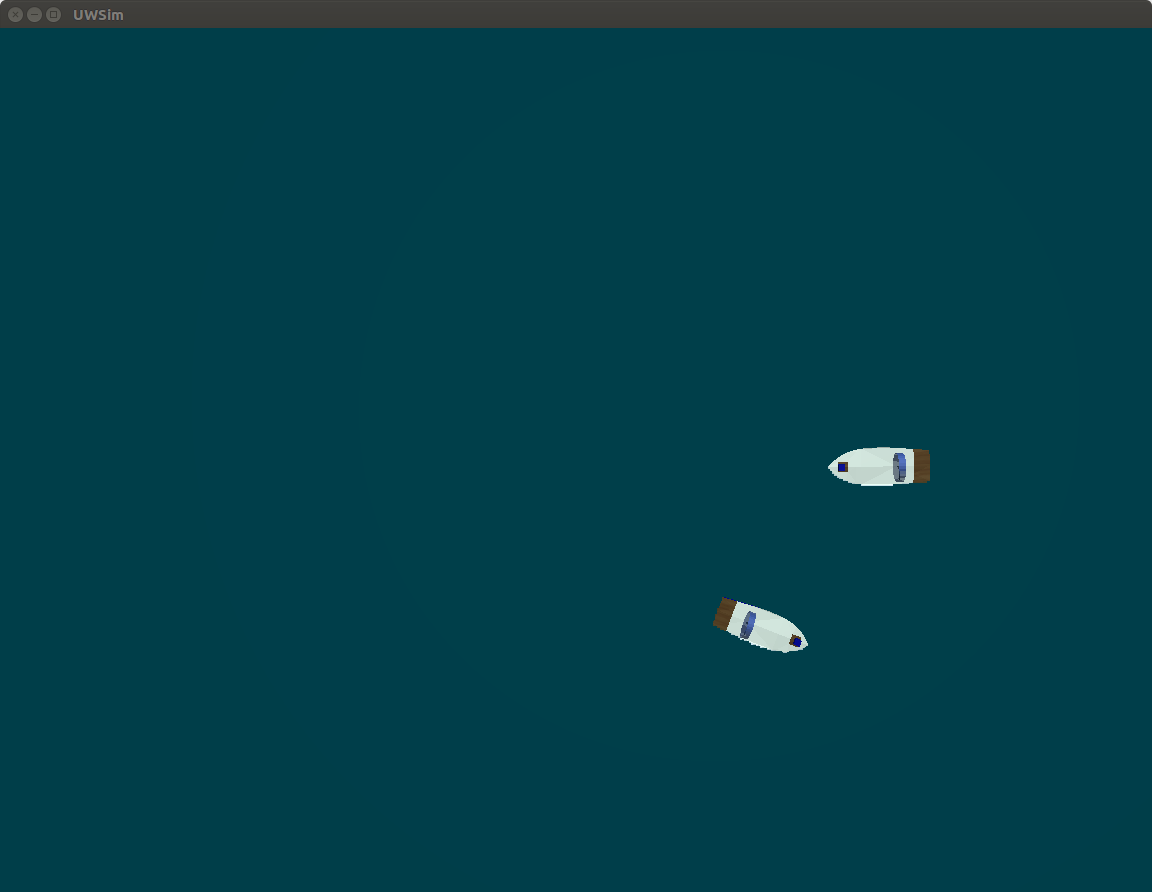
\includegraphics[scale=0.2]{figs/Experiment_HeadOn_5.png}\\
        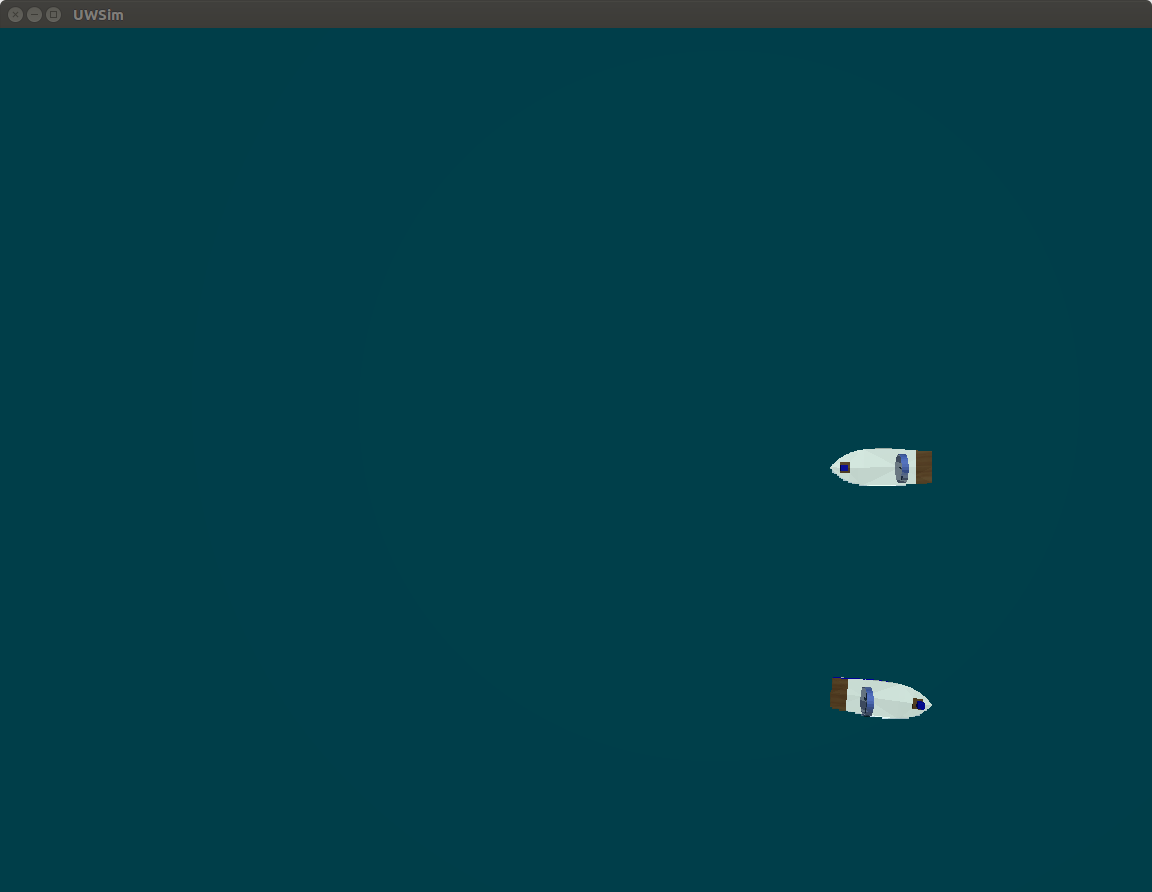
\includegraphics[scale=0.2]{figs/Experiment_HeadOn_6.png}
        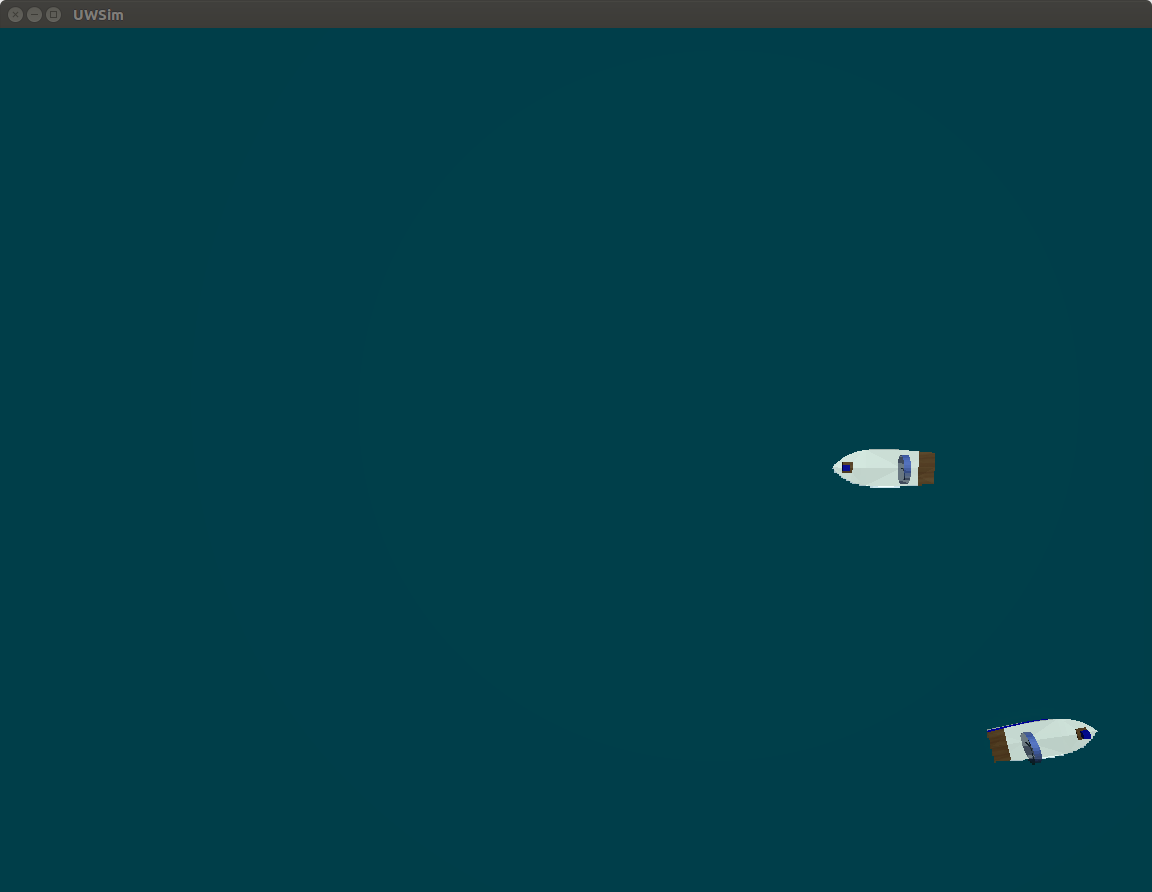
\includegraphics[scale=0.2]{figs/Experiment_HeadOn_7.png}
        \caption{USV motion from initial position to desired final location, avoiding collision with another ship}
        \label{fig:Experiment_HeadOn_Sequence}
    \end{figure}
    
    \section{Additional Information about Academic Progress }

    Below we present a summary of the current academic progress: 

    \begin{itemize}
        \item Already done credits: 17;
        \item Pending credits: 7 (\textit{Agentes Autônomos} - 2 credits, \textit{Visualização de Dados} - 2 credits, \textit{Planejamento de Experimentos para Sistemas Computacionais} - 2 credits, and textual production - 1 credit);
        \item Mandatory courses attended (\textit{Teoria da Computação} and \textit{Lógica e Álgebras Computacionais});
        \item Author of an already accepted Qualis A1 survey. Survey about the use of \ac{USV} on disaster scenarios, written with the research group of the \ac{LSA}.
        
        %AMA 31/1 agora vc pode dizer q foi aprovado :D
        % DJ: Done
    \end{itemize}